\chapter{Background}
% \chapter{Trabalhos Relacionados}

% In this chapter we will present the existing works about data analysis and
% outlier detection with algorithms and strategies of how to use this approach to improve the analysis of data and increase the amount and the quality of the  information that we can retrieve from datasets.

Neste capítulo nós vamos apresentar os trabalhos existentes sobre análise de dados e detecção de outliers com algoritmos e estratégias de como usar essa abordagem para melhorar a análise dos dados e aumentar a quantidade e a qualidade das informações que podemos obter dos datasets.

% \section{Related Work}
\section{Trabalhos Relacionados}

\subsection{GeoGuide}

% Pursuing improve the spatial data analysis and the guidance approach for this kind of data, the GeoGuide \cite{omidvarTehrani2017} is a interactive framework that aims to highlight to the analyst a subset of $k$ interesting spatial points, based on the analyst \textit{implicit} (e.g. mouse tracking) and \textit{explicit} (e.g. points clicked) feedbacks, that he may not seem because of the huge amount of information on his screen. This framework considers two metrics to give the subset highlight. The first one is the \textbf{relevance} of each point to the point selected by the analyst considering the attributes of those points. The second one is the geographically \textbf{diversity} to expand the analyst area in chase of possible new interesting regions.

Visando melhorar a análise de dados espaciais e a abordagem por orientação para esse tipo de dado, o GeoGuide \cite{omidvarTehrani2017} é um framework interativo que visa destacar para o analista um subconjunto de $k$ pontos espaciais interessantes, baseado nos feedbacks \textit{implícito} (ex.: rastreamento do mouse) e \textit{explícito} (ex.: pontos clicados) do analista, que podem não terem sido vistos dado o montante de informação aparente na sua tela. Esse framework leva em consideração duas importantes métricas para poder destacar um subconjunto. A primeira é a \textbf{relevância} de cada ponto para o ponto selecionado pelo analista considerando os atributos não espaciais desses pontos. O segundo é a \textbf{diversidade} geográfica para que assim possa expandir a área de análise do usuário em busca de possíveis novas regiões de seu interesse.

% All this process can be used in generic spatial datasets, as long as each point have two characteristics: geographical attributes (i.e. latitude and longitude) and metadata attributes about its own domain. For instance, the Airbnb\footnote{\it http://www.airbnb.com} platform has open datasets about the available home-stays to rent and each one has the geographical attributes and \textit{price, hostname, availability} as their metadata attributes that are specific for each dataset type as presented in Figure \ref{fig:geoguide-example-airbnb}. Using this approach, the GeoGuide is the first efficient interactive highlighting framework for spatial data, combining analyst feedbacks with relevance and diversity metrics to display to the analyst a set of interesting points that he may be not focused during his analysis.

Todo esse processo pode ser utilizado em datasets espaciais genéricos, contanto que cada ponto do conjunto tenha duas características: atributos geográficos (ex.: latitude e longitude) e atributos \textit{metadados} de domínio do dataset. Por exemplo, a plataforma Airbnb\footnote{\it http://www.airbnb.com} tem datasets abertos sobre as casa disponíveis para alugar e cada uma delas tem atributos geográficos e \textit{preço, nome do hospedados e disponibilidade} como seus atributos metadados que são específicos para cada tipo de dataset como podemos ver na Figura \ref{fig:geoguide-example-airbnb}. Utilizando essa abordagem, o GeoGuide é o primeiro framework interativo eficiente para destaque de dados espaciais, combinando o feedback do analista com as métricas de relevância e diversidade para mostrar a ele um subconjunto de pontos interessantes que podem não ter sido deixado de lado durante sua análise.

% \begin{figure*}[t]
% 	\centering
% 	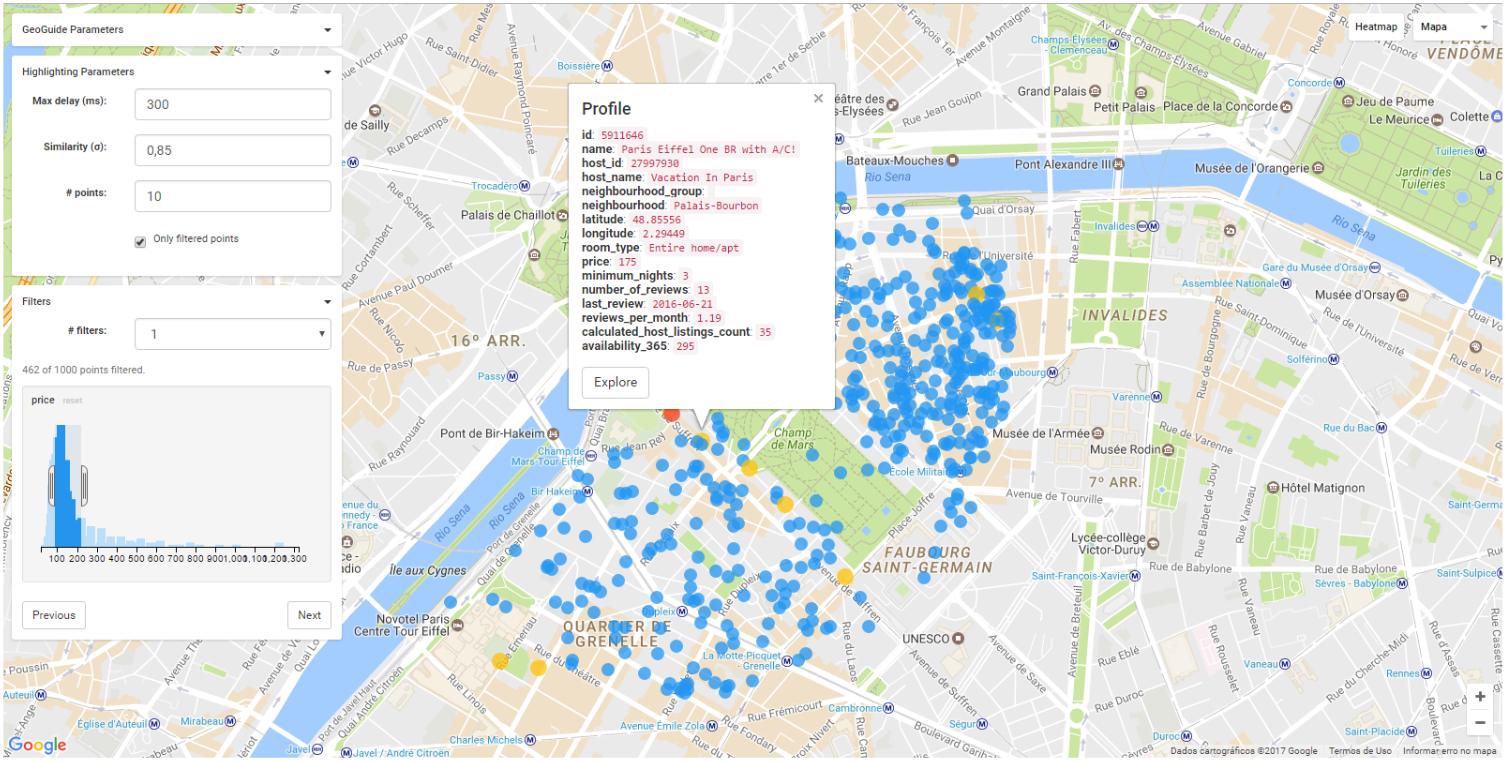
\includegraphics[width=\textwidth]{images/geoguide-example-airbnb}
% 	\caption{GeoGuide Image on Airbnb Dataset - Paris City}
% 	\label{fig:geoguide-example-airbnb}
% 	\vspace{-10pt}
% \end{figure*}
\begin{figure*}[t]
	\centering
	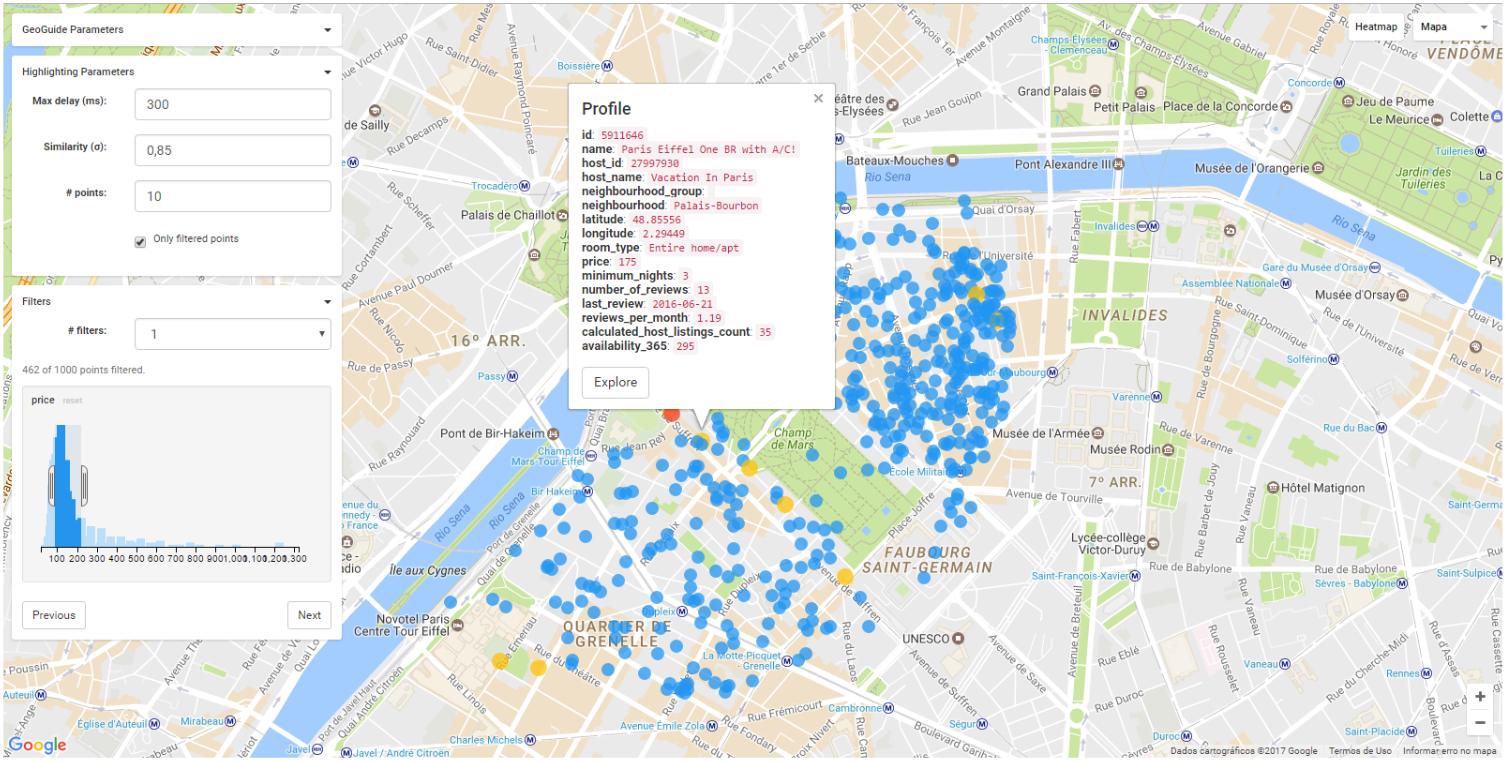
\includegraphics[width=\textwidth]{images/geoguide-example-airbnb}
	\caption{Imagem do GeoGuide no dataset do Airbnb - Cidade de Pais}
	\label{fig:geoguide-example-airbnb}
	\vspace{-10pt}
\end{figure*}

\subsection{Outliers}

% TODO: usar definição de Hawkins (procurar slide dos algoritmos de detecção de outlier)
% TODO: adicionar exemplos de outlier detection

% Outliers in the statistics area are when one finds ``aberrant values'' in a given series of data, that is when one finds an atypical value or with a great distance from the normal distribution in that set. For example, when a researcher wants to monitor the temperature of his CPU during a certain time interval and it has been realized that the temperature range is between 34 ºC and 45 ºC degrees being 48 ºC the maximum temperature and 27 ºC the minimum temperature and in the middle of this sample are some punctual registers of 0 ºC, this can be characterized as an outlier and, most likely, will be understood as a malfunction of the equipment that performed the collection of these CPU temperatures.

No campo da estatística, Outliers são quando se encontram ``valores aberrantes'' num determinado conjunto de dados, ou seja, quando alguém acha um valor atípico ou muito fora da distribuição normal daquele conjunto. Por exemplo, quando um pesquisador quer monitorar a temperatura de sua CPU durante um certo intervalo de tempo e foi percebido que a variação de temperatura foi entre 34 ºC e 45 ºC com máxima de 48 ºC e mínima de 27 ºC e no meio dessa amostragem são encontrados registros pontuais de 0 ºC, isso é caracterizado como um outlier a, muito provavelmente, será interpretado como um defeito do equipamento que realizou a coleta da temperatura da CPU.

% However, there are several ways to interpret an Outlier (not only as a collection error), but also as: data that belong to a different population of the sample, a damaged data, areas in which a certain theory is not valid or even, when the sample is too large, it is normal to have some small amounts of outliers in that group. In cases where it is proven that it is not the fault of a collection equipment malfunction or that it was not a human mistake, it is extremely important to know the why of that outlier and try to understand it, because it is not interesting for a research simply remove it from the sample or re-signify it by assigning a new value. This change may compromise the validity of the research, and if this is done, it is extremely important to document and record those changes.

Entretanto, existem diversas formas de interpretar um Outlier além de um erro da coleta, como: um dado que pertença à uma população diferente da amostra, um dado defeituoso, um dado que esteja numa área em que certa teoria não é válida ou até, quando a amostra é muito grande, é normal haver pequenos quantidades de outliers naquele grupo. Em casos em que são provados que não é culpa de um equipamento defeituoso de coleta ou que não foi uma falha humana, é extremamente importante entender o porquê daquele outlier, pois não é interessante para o pesquisador simplesmente removê-lo ou ressignificá-lo definindo-lhe um novo valor, já que essa mudança pode comprometer a validade da pesquisa e, caso aconteça, é de extrema importância que tudo isso seja documentado para registro dessas alterações.

% As the information technologies improve and continuously increase their computational power, a great variety of algorithms for outlier detection has been surging and applied in different contexts with diverse characteristics and the choice for one of those algorithms is based on the problem domain. Next section will present some of those algorithms with a brief explanation about each one.

Assim como as tecnologias da informação melhoram e aumentam continuamente seu poder computacional, uma grande variedade de algoritmos para detecção de outliers tem surgido e vem sendo aplicado em diferentes contextos com diversas características, sendo que a escolha para um desses algoritmos é baseada no domínio do problema. Na próxima seção nós apresentaremos alguns desses algoritmos com uma breve explicação sobre cada um.

% \section{Algorithms}
\section{Algoritmos}

\subsection{Z-Score}

% Z-Score is one of the simplest methods for detecting outliers in a dataset. It is a
% parametric method and takes into account only one attribute per execution. It is also
% necessary the input of a threshold (usually is a value between 2.5 to 3.5) to be able
% to define if a given data can be considered an outlier or not. This method is suitable
% for small datasets that follow the Gaussian distribution.

Z-Score é um dos métodos mais simples para detecção de outliers em um dataset. É um método parametrico que leva em consideração somente um atributo por execução e é necessário a entrada de um valor limite (geralmente um valor entre 2,5 e 3,5) para poder definir se um determinado dado pode ser considerado como um outlier ou não. Esse método é adequado para pequenos datasets que seguem a distribuição Gaussiana.

\subsection{DBSCAN}

% It is a density-based spatial clustering algorithm \cite{Ester:1996:DAD:3001460.3001507} that can be applied in datasets that cannot be presumed what their distribution. It accepts multidimensional datasets (with 3 or more dimensions). However, you need a parameter (MinPts) that defines how many minimum points are needed to form a cluster. Thus, if the size of the set change, this parameter will need to be updated, otherwise the DBSCAN can become inefficient.

É um algoritmo de clusterização de dados espaciais baseado em densidade \cite{Ester:1996:DAD:3001460.3001507} pode ser aplicado em datasets os quais não se pode presumir qual a sua distribuição e que aceita datasets multidimensionais (com 3 ou mais dimensões). Entretanto, é necessário a entrada de um parametro (MinPts) que definirá quantos pontos são minimamente necessários para se formar um \textit{cluster}. Portanto, se o tamanho do conjunto mudar, esse parâmetro terá que ser atualizado, caso contrário, o DBSCAN pode se tornar ineficiente.

\subsection{Isolation Forests}

% It is an algorithm of detection of outliers \cite{IsolationForests} that uses a concept of machine learning that
% is the decision tree. It is one-dimensional (only takes one attribute at a time) and is
% required few parameters (this facilitates the configuration and use of the algorithm).
% No need to climb your values and a very robust algorithm for large datasets.

É um algoritmo de detecção de outliers \cite{IsolationForests} que usa um dos conceitos de aprendizagem de máquina que são as chamadas árvores de decisão. É unidimensional (só leva em consideração um atributo por vez) e são necessários poucos parâmetros (isso facilita a configuração e uso do algoritmo). Por não precisar escalar seus valores para sua execução, isso o torna um algoritmo robusto para grandes datasets.


\subsection{FDC}

% It is a depth-based algorithm \cite{Johnson:1998:FCD:3000292.3000332} approach for detection of outliers in 2D datasets based on the concept of ISODEPTH algorithm. The FDC computes the first k 2D depth contours (the points that can be considered outliers) by restricting to a small part of the complete dataset. In this way, it is more efficient by not having to calculate in the complete dataset and thus scaling more easily for large datasets of two dimensions.

É uma abordagem de algoritmo baseado em profundidade \cite{Johnson:1998:FCD:3000292.3000332} para detecção de outliers em datasets 2D que se baseia no conceito do algoritmo ISODEPTH.
% TODO: referência algoritmo isodepth.
O FDC computa os primeiros $k$ contornos de profundidade (os pontos que podem ser considerados outliers) restrigindo a uma pequena parte do dataset completo. Dessa forma, é mais eficiente por não ter que calcular no dataset completo e, portanto, mais fácil de escalar para grandes datasets de duas dimensões.

\subsection{HOD}

% It is a distance-based outlier detection method \cite{Xu2016} that emerges to overcome the statistics-based
% concept because in the vast majority of datasets the probability distribution is not known.
% In this way, the method search for outliers based on their distance from their neighbors
% and if that point has a distance greater than a predefined parameter, then that point is
% considered an outlier. However, if there is a cluster of outliers in the dataset, this
% can affect its detection by distance-based algorithms, with this comes the concept of HOD
% (Hidden Outlier Detection) algorithms that aim to find outliers even when they are grouped
% and in enough quantity to form a cluster.

É um método de detecção de outlier baseado em distância \cite{Xu2016} que surge para superar os métodos baseados em estatísticas já que na vasta maioria dos datasets a distribuição de probabilidade não é conhecida. Dessa forma, o método busca por outliers baseado na sua distância em relação aos seus vizinhos e se essa distância é maior que um parâmetro de entrada predefinido, então esse ponto é considerado um outlier. Entretanto, se já existe um cluster de outliers no dataset, isso pode afetar a detecção em algoritmos baseado em distância, para isso que serve o conceito HOD (\textit{Hidden Outlier Detection}) do algoritmo que visa encontrar outliers mesmo quando eles estão agrupados em quantidades suficiente para formação de um cluster.

\subsection{ORCA}

% It is a distance-based algorithm \cite{Bay:2003:MDO:956750.956758} that optimizes a simple nested loop algorithm (which are logarithmic algorithms and extremely inefficient when dealing with large datasets) by removing possible non-outliers during their execution. This way, instead of processing the complete dataset by calculating all possible distances, it removes unnecessary calculations that would be executed if a non-outlier point were taken to the end. From him, new researches have emerged further refining this concept.

É um algoritmo baseado em distância \cite{Bay:2003:MDO:956750.956758} que otimiza um algoritmo simples de loop aninhado 
% TODO: pegar referência de nested loop
(que são algoritmos de complexidade exponencial os quais são extremamente ineficientes quando utilizados em grandes datasets) pela remoção de possíveis \textit{non-outliers} durante sua execução. Dessa forma, ao invés de processar o dataset por completo, ele vai removendo cálculos que serão desnecessários, já que o ponto não vai ser considerado um outlier. A partir dele, novas pesquisas têm surgido para refinar mais esse conceito. 

\subsection{Linearization}

% It is a distance-based algorithm \cite{10.1007/3-540-45681-3_2} that detects outliers by calculating the sum of the distances of a point in relation to its neighbor, calling it weight, and setting an outlier as the points with the greatest weights in the dataset. In this way, it is an efficient algorithm and it is linearly scaled both in the number of points and in the number of dimensions. To calculate these outliers more efficiently the algorithm uses the concept of the Hilbert space-filling curve.

É um algoritmo baseado em distância \cite{10.1007/3-540-45681-3_2} que detecta outliers calculando a soma das distâncias de um ponto em relação aos seus vizinhos, chamando isso de \textit{peso}, e definindo os outliers como os pontos com os maiores pesos no dataset. Dessa forma, é um algoritmo eficiente de complexidade linear tanto em relação ao número de pontos como ao número de dimensões. Para ajudar a calcular esses outliers mais eficientemente, o algoritmo utiliza o conceito da \textit{curva de Hilbert}
% TODO: adicionar referência à curva de Hilbert 

\subsection{RBRP}

% It is an algorithm for high-performance multidimensional datasets that is based on distances between the points to be able to define what the outliers are \cite{Ghoting2006}. Its difference to the other distance-based algorithms is that it is more efficient for datasets with multiple dimensions and in comparisons with others, its scalability is approximately linear for the number of dimensions and logarithmic for the number of points in the dataset.

É um algoritmo de alta perfomance para datasets multidimensionais que é baseado nas distâncias entre os pontos para poder definir quais são os outliers no dataset \cite{Ghoting2006}. Sua diferença para os outros algoritmos baseado em distância é que ele se torna mais eficiente quando executado em dataset com múltiplas dimensões, sua escalabilidade é aproximadamente linear para o número de dimensões e logarítmica para o número de pontos no dataset.

\subsection{LOF}

% It is a density-based algorithm that adds a new concept in the search for outliers: the Local Outlier Factor (LOF) \cite{Breunig:2000:LID:335191.335388}, which is a degree of propensity to be an outlier so that the process of outlier definition is not more binary, but something gradual. With this, the approach is not to define whether a point is an outlier or not, but rather the ``how outlier'' that point is in that dataset. The outlier factor is local in the sense that only a neighborhood of that point is taken into account to define its factor.

É um algoritmo baseado em densidade que adiciona um novo conceito na busca por outliers: o \textit{Local Outlier Factor (LOF)} \cite{Breunig:2000:LID:335191.335388}, que é um grau de propensidade que aquele ponto tem de ser um outlier e dessa forma o processo de definição de outlier não é mais binário, mas sim algo gradual. Com isto, a abordagem não é mais sobre um ponto ser outlier ou não, mas sim o ``quão outlier'' esse ponto é em relação ao dataset. O \textit{outlier factor} é local no sentido que somente os vizinhos daquele ponto é levado em consideração para definir seu fator.

\subsection{ABOD}

% It is an angle-based algorithm \cite{Kriegel:2008:AOD:1401890.1401946} for detection of outliers that is focused on high-dimensional datasets, different from other distance-based algorithms that end up damaged when one has many dimensions. Your approach is based on the calculation of a degree of angle between the different vectors of a point with its neighbors. With this, more centralized points within the cluster will have this degree calculated with a high value, the points more on the edge of the clusters will have this degree a little smaller and the possible outliers will have that degree with a very small value, since they will generally be far from the cluster in a particular direction.

É um algoritmo de detecção de outlier baseado em ângulo \cite{Kriegel:2008:AOD:1401890.1401946} que é focado em datasets de altas dimensões, diferente de outros algoritmos baseado em distãncia que acabam prejudicados quando o dataset tem muitas dimensões. Sua abordagem é baseado no cálculo do grau do ângulo entre os diferentes vetores de um ponto com os seus vizinhos. Com isto, pontos mais centralizados dentro do cluster terão esse grau calculado com um valor maior, já os pontos mais próximos da borda terão esse valor um pouco menor e o possíveis outliers terão esse grau com valores muito pequenos, já que eles geralmente estarão distantes do cluster em uma direção particular. 

\vspace{25pt}

% Based on the algorithms presented, we organize each one according the answer of proposed questions about outlier detection algorithms in general. The proposed questions are: \textbf{I} \textit{Is it parametric?}; \textbf{II} \textit{Which is the approach?}; \textbf{III} \textit{Is it scalable in performance terms?}; \textbf{IV} \textit{Is it multidimensional scalable?} and \textbf{V} \textit{Does it receive any argument?}. The result is presented in the Table \ref{table:algorithms-comparison}.

Baseado nos algoritmos apresentados, nós organizamos cada um de acordo com a resposta para nossas questões propostas sobre algoritmos de detecção de outliers no geral. As questões são: \textbf{I} \textit{É paramétrico?}; \textbf{II} \textit{Qual é a abordagem?}; \textbf{III} \textit{É escalável em termos de performance?}; \textbf{IV} \textit{É escalável em termos de múltiplas dimensões?} e \textbf{V} \textit{Ele recebe algum argumento?}. O resultado é apresentado na Tabela Table \ref{table:algorithms-comparison}.

\begin{table}[]
	\centering
	\begin{tabular}{|l|l|l|l|l|l|}
		\hline
		\textbf{Algorithms}               & \textbf{I} & \textbf{II}             & \textbf{III} & \textbf{IV} & \textbf{V} \\ \hline
		\textbf{Z-Score}                  & Sim        & Baseado em Modelo       & Não          & Não         & Sim        \\ \hline
		\textbf{DBSCAN}                   & Não        & Baseado em Densidade    & Não          & Sim         & Sim        \\ \hline
		\textbf{Isolation Forests}        & Não        & Baseado em Profundidade & Não          & Não         & Não        \\ \hline
		\textbf{FDC}                      & Não        & Baseado em Profundidade & Sim          & Não         & Não        \\ \hline
		\textbf{Hidden Outlier Detection} & Não        & Baseado em Distância    & Sim          & Sim         & Sim        \\ \hline
		\textbf{ORCA}                     & Não        & Baseado em Distância    & Não          & Sim         & Sim        \\ \hline
		\textbf{Linearization}            & Não        & Baseado em Distância    & Sim          & Sim         & Sim        \\ \hline
		\textbf{RBRP}                     & Não        & Baseado em Distância    & Sim          & Sim         & Sim        \\ \hline
		\textbf{LOF}                      & Não        & Baseado em Densidade    & Não          & Sim         & Sim        \\ \hline
		\textbf{ABOD}                     & Não        & Altas Dimensões         & Não          & Sim         & Não        \\ \hline
	\end{tabular}
	\caption{Comparação dos Algoritmos de Detecção de Outlier apresentados}
	\label{table:algorithms-comparison}
\end{table}

% Each question has a specific reason to be in the Table \ref{table:algorithms-comparison}. The question \textbf{I} is about the probability distribution of the dataset. If the algorithm is parametric, so we can assume a probability distribution based on a fixed set of parameters. The question \textbf{II} serves to classify each algorithm based on his approach for detect a data as an outlier or not, the options are: \textit{Model Based}, \textit{Density Based}, \textit{Depth Based}, \textit{Distance Based}, \textit{High Dimensional}. The question \textbf{III} is relative to the performance of each algorithm, if the algorithm execution time is not compromised as the input data increase, it means the algorithm is scalable in perfomance terms. The question \textbf{IV} is about the performance of each algorithm too, but in this case is related to the perfomance when the dimension of the data increase. At least, the question \textbf{V} indicates if the algorithm require any input argument to process the dataset, this is important because if it requires many arguments, this can be a accuraccy problem when the dataset increase.

Cada questão tem uma motivação específica para estar na Tabela \ref{table:algorithms-comparison}. A questão \textbf{I} é sobre a distribuição de probabilidade do dataset. Se o algoritmo é paramétrico, então nós podemos assumir a distribuição de probabilidade do dataset baseado em um conjunto fixo de parâmetros. A questão \textbf{II} serve para classificar cada algoritmo baseado na abordagem que ele utiliza para indicar se um dado é um outlier ou não, as opções são: textit{Baseado em Modelo}, \textit{Baseado em Densidade}, \textit{Baseado em Profundidade}, \textit{Baseado em Distância} e \textit{Altas Dimensões}. A questão \textbf{III} é relativa a performance computacional de cada algoritmo, se o tempo de execução do algoritmo não é comprometido de acordo com o crescimento do dataset, significa que ele é escalável em termos de performance. A questão \textbf{IV} é sobre a performance de cada algoritmo também, mas nesse caso é relacionado ao crescimento de dimensões do dataset. Por fim, a questão \textbf{V} indica se o algoritmo requer algum argumento de entrada para processar o dataset, isso é importante pois se o algoritmo requer muitos argumentos pode se tornar um problema de precisão quando o dataset aumentar.